\chapter{GSI Applications for Regional 3DVar, Hybrid 3DEnVar and Hybrid 4DEnVar}\label{gsi_reg}
\setlength{\parskip}{12pt}

In this chapter, information from the previous chapters will be applied to three regional GSI cases with different data sources. These examples are to give users a clear idea of how to set up GSI with various configurations and properly check the run status and analysis results in order to determine if a particular GSI application was successful. Note that the examples here only use the WRF-ARW system - WRF-NMM runs are similar, but require different background and namelist options. 

For illustrations of all the cases, it is assumed that the reader has successfully compiled GSI on a local machine. For regional case studies, users should have the following data available:

\begin{enumerate}
\item Background file
\begin{itemize}
\item When using WRF, WPS and real.exe will be run to create a WRF input file: wrfinput\_<domain>\_<yyyy-mm-dd\_hh:mm:ss>
\end{itemize}
\item Conventional data

\begin{itemize}
\item Real time NAM PrepBUFR data can be obtained from the server:

\url{ftp://ftpprd.ncep.noaa.gov/pub/data/nccf/com/nam/prod}

\textit{Note: An NDAS PrepBUFR file was chosen to increase the amount of data used in the analysis (compared to a NAM PrepBUFR file) }
\end{itemize}

\item Radiance data and GPS RO data

\begin{itemize}
\item Real time GDAS BUFR files can be obtained from the following server:

\url{ftp://ftpprd.ncep.noaa.gov/pub/data/nccf/com/gfs/prod}

\textit{Note: GDAS data was chosen to get better coverage for radiance and GPS/RO refractivity}
\end{itemize}

\end{enumerate}

The following cases will give users an example of a successful GSI run with various data sources.  Users are welcome to download these example data from the GSI users\textquotesingle \ webpage (online case) or create a new background and get the observational data from the above server.  The background and observations used in this case study are as follows:

\begin{enumerate}
\item Background files: wrfinput\_d01\_2014-06-17\_00:00:00
\begin{itemize}
\item The horizontal grid spacing is 30-km with 51 vertical sigma levels
\begin{figure}[h!]
  \begin{minipage}[t]{0.5\linewidth}
  \centering
  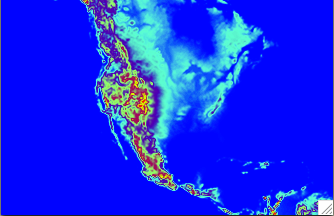
\includegraphics[width=0.7\textwidth]{images/terrain}
  \end{minipage} %
  \begin{minipage}[t]{0.5\linewidth}
  \centering
  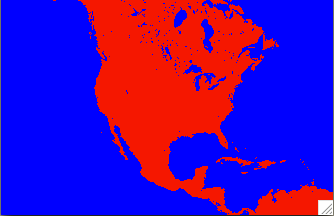
\includegraphics[width=0.7\textwidth]{images/landmask}
  \end{minipage}
  \caption{The terrain (left) and land mask (right) of the background used in this case study.}
  \label{fig:terland}
\end{figure}
\end{itemize}
\item Conventional data: NAM PrepBUFR data from 0000 UTC 17 June 2014
\begin{itemize}
\item File: \textit{nam.t00z.prepbufr.tm00.nr}
\end{itemize}
\item Radiance and GPS RO data: GDAS PREPBUFR data from 0000 UTC 17 June 2014
\begin{itemize}
\item Files: \textit{gdas.t00z.1bamua.tm00.bufr\_d}

     \qquad\quad  \textit{gdas.t00z.1bhrs4.tm00.bufr\_d}

     \qquad\quad  \textit{gdas.t00z.gpsro.tm00.bufr\_d}
\end{itemize}
\end{enumerate}

This case study was run on a Linux cluster. As of  version 3.2, the BUFR/PrepBUFR files do not need to be byte-swapped to little endian format. BUFRLIB can automatically handle byte order issues.

Assume the background file is located at:

\textit{data/2014061700/arw}

All the observations are located at:

\textit{data/2014061700/obs}

And the GSI release version 3.6 is located at:

\textit{code/comGSI(version\_number)\_EnKF(version\_number)}

%-------------------------------------------------------------------------------
\section{Assimilating Conventional Observations with Regional GSI}
%-------------------------------------------------------------------------------

%-------------------------------------------------------------------------------
\subsection{Run Script}
\label{sec5.1.1}
%-------------------------------------------------------------------------------

With GSI successfully compiled and background and observational data acquired, move to the \textit{./run} directory under \textit{./comGSIv3.5\_EnKFv1.1} to run the GSI using the sample script \textit{run\_gsi\_regional.ksh}.  The \textit{run\_gsi\_regional.ksh} script must be modified in several places before running:

\begin{itemize}
\item Set up batch queuing system. \\
To run GSI with multi-processors, a job queuing section has to be added at the beginning of the \textit{run\_gsi\_regional.ksh} script.  The set up of the job queue is dependent on the machine and the job control system.  More setup examples are described in section \ref{sec3.2.2}. The following example is set up to run on a Linux cluster supercomputer with LSF. The job section is as follows:
 
\begin{scriptsize}
\begin{verbatim}
#BSUB -P ?????????             # project code
#BSUB -W 00:20                 # wall-clock time (hrs:mins)
#BSUB -n 4                     # number of tasks in job         
#BSUB -R "span[ptile=16]"      # run 16 MPI tasks per node
#BSUB -J gsi                   # job name
#BSUB -o gsi.%J.out         
#BSUB -e gsi.%J.err 
#BSUB -q small                 # queue
\end{verbatim}
\end{scriptsize}

In order to find out how to set up the job section, a good method is to use an existing MPI job script and copy the job section over. 
\\

\item Set up the number of processors and the job queue system used.  For this example, LINUX\_PBS and four processors are used:

\begin{scriptsize}
\begin{verbatim}
GSIPROC=4
ARCH='LINUX_PBS'
\end{verbatim}
\end{scriptsize}

\item Set up the case data, analysis time, GSI fix files, GSI executable, and CRTM coefficients:

Set up analysis time: 

\begin{scriptsize}
\begin{verbatim}
ANAL_TIME=2014061700
\end{verbatim}
\end{scriptsize}

Set up a working directory, which will hold all the analysis results.  This directory must have correct write permissions, as well as enough space to hold the output. 

\begin{scriptsize}
\begin{verbatim}
WORK_ROOT=/scratch1/gsiprd_${ANAL_TIME}_prepbufr
\end{verbatim}
\end{scriptsize}

Set path to the background directory and file: 

\begin{scriptsize}
\begin{verbatim}
  BK_ROOT=data/20140617/${ANAL_TIME}/arw
  BK_FILE=${BK_ROOT}/wrfinput_d01.${ANAL_TIME}
\end{verbatim}
\end{scriptsize}

Set path to the observation directory and the PrepBUFR file within the observation directory. All observations to be assimilated should be in the observation directory. 

\begin{scriptsize}
\begin{verbatim}
  OBS_ROOT=data/20140617/${ANAL_TIME}/obs
  PREPBUFR=${OBS_ROOT}/nam.t${HH}z.prepbufr.tm00.nr
\end{verbatim}
\end{scriptsize}

Set up the GSI system used for this case, including the paths of fix files and the CRTM coefficients as well as the location of the GSI executable and the namelist file: 

\begin{scriptsize}
\begin{verbatim}
  CRTM_ROOT=data/fix/CRTM_2.2.3
  GSI_ROOT=/comGSIv3.5_EnKFv1.1
  FIX_ROOT=${GSI_ROOT}/fix
  GSI_EXE=${GSI_ROOT}/run/gsi.exe
  GSI_NAMELIST=${GSI_ROOT}/run/comgsi_namelist.sh
\end{verbatim}
\end{scriptsize}

\item Set which background and background error file to use:

\begin{scriptsize}
\begin{verbatim}
bk_core=ARW
bkcv_option=NAM
if_clean=clean 
\end{verbatim}
\end{scriptsize}

This example uses the ARW NetCDF background; therefore \verb|bk_core| is set to 'ARW.'  The regional background error covariance file is used in this case, as set by \verb|bkcv_option=NAM|.  Finally, the run scripts are set to clean the run directory to delete all temporary intermediate files.
\end{itemize}

%-------------------------------------------------------------------------------
\subsection{Run GSI and Check the Run Status}
\label{sec5.1.2}
%-------------------------------------------------------------------------------

Once the run script is set up properly for the case and machine, and the anavinfo file has been updated with the same number of vertical levels as the background (please see section \ref{sec3.1} for more details), GSI can be run through the run script. On our test machine, the GSI run is submitted as follows:

\begin{scriptsize}
\begin{verbatim}
$ bsub < run_gsi_regional.ksh
\end{verbatim}
\end{scriptsize}

While the job is running, move to the working directory and check the details. Given the following working directory setup:

\begin{scriptsize}
\begin{verbatim}
 WORK_ROOT=/scratch1/gsiprd_${ANAL_TIME}_prepbufr
\end{verbatim}
\end{scriptsize}

Go to directory \textit{/scratch1} to check the GSI run directory.

A directory named \textit{gsiprd\_2014061700\_prepbufr} should have been created.  This directory is the run directory for this GSI case study.  While GSI is still running, the contents of this directory should include files such as:

\begin{scriptsize}
\begin{verbatim}
imgr_g12.TauCoeff.bin        	ssmi_f15.SpcCoeff.bin
imgr_g13.SpcCoeff.bin        	ssmi_f15.TauCoeff.bin
imgr_g13.TauCoeff.bin        	ssmis_f16.SpcCoeff.bin
\end{verbatim}
\end{scriptsize}

These are CRTM coefficient files that have been linked to this run directory through the GSI run script.  Additionally, many other files are linked or copied to this run directory or generated during the run, such as:

\begin{itemize}
\item \verb|stdout|:		standard output file
\item \verb|wrf_inout|:  	background file
\item \verb|gsiparm.anl|:   	GSI namelist
\item \verb|prepbufr|:  	prepBUFR file for conventional observation
\item \verb|convinfo|: 		data usage control for conventional data
\item \verb|berror_stats|: 	background error file
\item \verb|errtable|: 		observation error file
\end{itemize}

The presence of these files indicates that the GSI run scripts have successfully set up a run environment for GSI and that the GSI executable is running.  While GSI is still running, checking the content of the standard output file (\textit{stdout}) can monitor the status of the GSI analysis:

\begin{tiny}
\begin{verbatim}
$ tail  stdout
[mhu@yslogin2 testarw_conv]$ tail stdout
pcgsoi: gnorm(1:2),b=  4.971613638691962543E-04  4.971613637988174387E-04  6.539937387039491679E-01
cost,grad,step,b,step? =   2  21  2.283071832605468444E+04  2.229711559527815246E-02  4.235685495878949780E+01  6.539937387039491679E-01  good 
pcgsoi: gnorm(1:2),b=  2.427998455757554152E-04  2.427998455925739387E-04  4.883723137754825139E-01
cost,grad,step,b,step? =   2  22  2.283069726786290266E+04  1.558203598942562579E-02  5.370146211199837438E+01  4.883723137754825139E-01  good 
pcgsoi: gnorm(1:2),b=  1.349871612172568163E-04  1.349871612633241600E-04  5.559606553423739328E-01
cost,grad,step,b,step? =   2  23  2.283068422915619885E+04  1.161839753224414365E-02  6.137769018004394894E+01  5.559606553423739328E-01  good 
pcgsoi: gnorm(1:2),b=  9.116990149652581994E-05  9.116990145686963470E-05  6.753968350377786978E-01
cost,grad,step,b,step? =   2  24  2.283067594395604101E+04  9.548293119533240308E-03  5.219011413742769179E+01  6.753968350377786978E-01  good 
pcgsoi: gnorm(1:2),b=  5.783146215365002791E-05  5.783146214669085264E-05  6.343262545796939378E-01
cost,grad,step,b,step? =   2  25  2.283067118578847294E+04  7.604700004184913528E-03  5.599317818817987558E+01  6.343262545796939378E-01  good 
\end{verbatim}
\end{tiny}

The above output shows that GSI is in the inner iteration stage.  It may take several minutes to finish the GSI run.  Once GSI has finished running, the number of files in the directory will be greatly reduced from those during the run stage.  This is because the run script was set to clean the working directory after a successful run.  The important analysis result files and configuration files will remain. Please check Section \ref{sec3.3} for more details on GSI run results. Upon successful completion of GSI, the run directory will look as follows:

\begin{scriptsize}
\begin{verbatim}

anavinfo                  fort.202  fort.214  fort.228                satbias_ang.out
berror_stats              fort.203  fort.215  fort.229                satbias_in
convinfo                  fort.204  fort.217  fort.230                satbias_out
diag_conv_anl.2014061700  fort.205  fort.218  gsi.exe                 satbias_out.int
diag_conv_ges.2014061700  fort.206  fort.219  gsiparm.anl             satbias_pc
errtable                  fort.207  fort.220  l2rwbufr                satbias_pc.out
fit_p1.2014061700         fort.208  fort.221  list_run_directory      satinfo
fit_q1.2014061700         fort.209  fort.223  ozinfo                  stdout
fit_rad1.2014061700       fort.210  fort.224  pcpbias_out             stdout.anl.2014061700
fit_t1.2014061700         fort.211  fort.225  pcpinfo                 wrfanl.2014061700
fit_w1.2014061700         fort.212  fort.226  prepbufr                wrf_inout
fort.201                  fort.213  fort.227  prepobs_prep.bufrtable
\end{verbatim}
\end{scriptsize}

%-------------------------------------------------------------------------------
\subsection{Check for Successful GSI Completion}
\label{sec5.1.3}
%-------------------------------------------------------------------------------

It is important to always check for a successful completion of the GSI analysis. However, completion of the GSI run without crashing does not guarantee a successful analysis.  First, it is necessary to check the \textit{stdout} file in the run directory to make sure GSI completed each step without any obvious problems.  The following are several important steps to check:

\begin{enumerate}
\item Read in the anavinfo and namelist files\\

The following lines show that GSI started normally and has read in the anavinfo and namelist files:
\begin{scriptsize}
\begin{verbatim}
 gsi_metguess_mod*init_:  2D-MET STATE VARIABLES:
 ps
 z
 gsi_metguess_mod*init_:  3D-MET STATE VARIABLES:
 u
 v
         ... ... 
         
 control_vectors*init_anacv: ALL CONTROL VARIABLES
 sf                              vp
 ps                              t
 q                               oz
         ... ...
         
 GSI_4DVAR:  nobs_bins =            1
 SETUP_4DVAR: l4dvar= F
 SETUP_4DVAR: l4densvar= F
 SETUP_4DVAR: winlen=   3.00000000000000
 SETUP_4DVAR: winoff=   3.00000000000000
 SETUP_4DVAR: hr_obsbin=   3.00000000000000
 SETUP_4DVAR: nobs_bins=           1

   ... ...
   
 &SETUP
 GENCODE =   78.0000000000000     ,
 FACTQMIN        =  0.000000000000000E+000,
 FACTQMAX        =  0.000000000000000E+000,
 CLIP_SUPERSATURATION    = F,
 FACTV   =   1.00000000000000     ,
 FACTL   =   1.00000000000000     ,
 FACTP   =   1.00000000000000     ,
 FACTG   =   1.00000000000000     ,

  ... ... 
\end{verbatim}
\end{scriptsize}
\item Read in the background field\\

The following lines in standard output file, immediately following the namelist section, indicate that GSI is reading the background fields.  Checking the range of the 'max' and 'min' values will indicate if certain background fields are normal. 

\begin{scriptsize}
\begin{verbatim}

  dh1  =            3
  iy,m,d,h,m,s=        2014           6          17           0           0
           0
  dh1  =            3
 RMS errore_var = SMOIS
 ndim1 =            3
 ordering = XYZ
 staggering =  N/A
 start_index =            1           1           1           0
 end_index =          332         215           4           0
 WrfType =          104
 ierr  =            0
  RMS errore_var = T ndim1 =            3  dh1 =            3

...............

  RMS errore_var = U ndim1=           3
  WrfType =          104  WRF_REAL=         104 ierr  =            0
  ordering = XYZ staggering =  N/A
  start_index =            1           1           1           0  end_index =
         333         215          50           0
  k,max,min,mid U=           1   18.50961      -17.84097     -0.8667576
  k,max,min,mid U=           2   18.68178      -18.39229     -0.8647658
  k,max,min,mid U=           3   19.28049      -19.42709     -0.8610985
  k,max,min,mid U=           4   19.60607      -21.29182     -0.8547171
  k,max,min,mid U=           5   21.58153      -24.50086     -0.8405453
\end{verbatim}
\end{scriptsize}

\item Read in observational data\\

Skipping through a majority of the content towards the middle of the standard output file, the following lines will appear:

\begin{scriptsize}
\begin{verbatim}
OBS_PARA: ps                        1429      3190      4655      6774
OBS_PARA: t                         2564      5200      7057     11128
OBS_PARA: q                         2346      4626      6148      8128
OBS_PARA: pw                          65        80        63        49
OBS_PARA: uv                        3358      6453      8091     11998
\end{verbatim}
\end{scriptsize}

This table is an important step to check if the observations have been read in, which types of observations have been read in, and the distribution of observations in each sub domain.  At this point, GSI has read in all the data needed for the analysis.  Following this table is the inner iteration information.\\ 

\item Inner iteration\\

The inner iteration step in the standard output file will look like this:

\begin{tiny}
\begin{verbatim}
 GLBSOI:  START pcgsoi jiter=           1
pcgsoi: gnorm(1:2),b=  1.131520548923311509E+02  1.131520548923311509E+02  0.000000000000000000E+00
 Begin J table inner/outer loop           0           1
     J term                                     J
surface pressure             5.7012207042385944E+03
temperature                  6.4242087278840627E+03
wind                         1.6782607330525603E+04
moisture                     3.5878183830232451E+03
 -----------------------------------------------------
 J Global                    3.2495855145671507E+04
 End Jo table inner/outer loop           0           1
Initial cost function =  3.249585514567150676E+04
Initial gradient norm =  1.063729546888358080E+01
cost,grad,step,b,step? =   1   0  3.249585514567150676E+04  1.063729546888358080E+01  2.548553547231620442E+01  0.000000000000000000E+00  good
pcgsoi: gnorm(1:2),b=  9.711890653545569307E+01  9.711890653545563623E+01  8.583043995786756586E-01
cost,grad,step,b,step? =   1   1  2.961211443694752961E+04  9.854892517701838273E+00  2.514521805501437157E+01  8.583043995786756586E-01  good
pcgsoi: gnorm(1:2),b=  8.597091659074136771E+01  8.597091659074150982E+01  8.852129791983981422E-01
cost,grad,step,b,step? =   1   2  2.717003835484893352E+04  9.272050290563644381E+00  1.036575164309021346E+01  8.852129791983981422E-01  good
pcgsoi: gnorm(1:2),b=  5.683515872824821002E+01  5.683515872824790449E+01  6.610975081120487040E-01

...
\end{verbatim}
\end{tiny}

Following the namelist set up, similar information will be repeated for each inner loop.  In this case, two outer loops with 50 inner loops in each outer loop are shown.  The last iteration looks like this:

\begin{tiny}
\begin{verbatim}
...
cost,grad,step,b,step? =   2  43  2.283066393607995633E+04  1.877001128106250809E-04  2.191568845986752123E+01  1.034537274286373876E+00  good
pcgsoi: gnorm(1:2),b=  1.819672329827284049E-08  1.819678976283112548E-08  5.164945106960998622E-01
cost,grad,step,b,step? =   2  44  2.283066393530783535E+04  1.348952308210814343E-04  4.180909725254741716E+01  5.164945106960998622E-01  good
pcgsoi: gnorm(1:2),b=  1.127913513618353988E-08  1.127903191777782680E-08  6.198386233002942669E-01
cost,grad,step,b,step? =   2  45  2.283066393454704667E+04  1.062032727187987424E-04  2.399192596022169610E+01  6.198386233002942669E-01  good
 PCGSOI: WARNING **** Stopping inner iteration ***
 gnorm  0.996812222890348903E-10 less than  0.100000000000000004E-09
 update_guess: successfully complete
\end{verbatim}
\end{tiny}

At the 45th iterationi, GSI met the stop threshold before getting to the maximum iteration number (50).  As a quick check, the J value should descend with each iteration.  Here, J has a value of 3.249585514567150676E+04 at the beginning and a value of 2.283066393454704667E+04 for the final iteration.  Therefore, the value has reduced by about one third, which is an expected reduction.\\

\item Write out analysis results\\

The final step of the GSI analysis procedure looks very similar to the portion where the background fields were read in:

\begin{scriptsize}
\begin{verbatim}
 ... ...

  max,min psfc=   102799.9       66793.78
  max,min MU=   2799.898      -1195.195
  RMS errore_var=MU
  ordering=XY
  WrfType,WRF_REAL=         104         104
  ndim1=           2
  staggering= N/A
  start_index=           1           1           1           0
  end_index1=         332         215          50           0
  k,max,min,mid T=           1   321.6157       270.8151       309.3634
  k,max,min,mid T=           2   321.7112       270.9660       309.4070
  k,max,min,mid T=           3   321.4324       271.2166       309.3831
  k,max,min,mid T=           4   321.2418       271.6100       309.3864
  k,max,min,mid T=           5   321.6863       272.2831       309.3308
  k,max,min,mid T=           6   320.9441       272.8387       309.1977
  k,max,min,mid T=           7   320.8511       273.1703       309.0908

   ... ...
\end{verbatim}
\end{scriptsize}

\item As an indication that GSI has successfully run, several lines will appear at the bottom of the file:

\begin{scriptsize}
\begin{verbatim}
     ENDING DATE-TIME    JUL 05,2016  11:30:38.156  187  TUE   2457575
     PROGRAM GSI_ANL HAS ENDED.
* . * . * . * . * . * . * . * . * . * . * . * . * . * . * . * . * . * . * . * .
\end{verbatim}
\end{scriptsize}

After carefully investigating each portion of the standard output file, it can be concluded that GSI successfully ran through every step and there were no run issues. A more complete description of the standard output file can be found in Section \ref{sec4.1}. However, it cannot be concluded that GSI successfully produced an analysis until more diagnosis has been completed.

\end{enumerate}

%-------------------------------------------------------------------------------
\subsection{Diagnose GSI Analysis Results}
%-------------------------------------------------------------------------------

%-------------------------------------------------------------------------------
\subsubsection{Check Analysis Fit to Observations}
%-------------------------------------------------------------------------------

The analysis uses observations to correct the background fields to fit to the observations under certain constraints.  The easiest way to confirm the GSI analysis results fit the observations better than the background is to check a set of files with names \textit{fort.2??}, where ?? is a number from 01 to 19 or larger than 20.  In the run scripts, several "fort" files have also been renamed as \textit{fit\_t1} (\textit{q1}, \textit{p1}, \textit{rad1}, \textit{w1}).\textit{YYYYMMDDHH}.  Please check Section \ref{sec4.5.1} for a detailed explanation of the fit files. Here, we illustrate how to use these fit files. 

\begin{itemize}[leftmargin=*]
\item \textit{fit\_t1.2014061700} (\textit{fort.203})

This file shows how the background and analysis fields fit to temperature observations.  The contents of this file show five data types were used in the analysis: 120, 130, 132, 180, and 182.  Also included are the number of observations, bias, and RMS error of observation minus background (o-g 01) or analysis (o-g 03) on each level for the three data types.  The following is part of the file, only showing data types 120 and 180:

\begin{tiny}
\begin{verbatim}

                              ptop   1000.0    900.0    800.0    600.0    400.0    300.0    250.0    200.0    150.0    100.0     50.0      0.0
     it     obs    type styp  pbot   1200.0   1000.0    900.0    800.0    600.0    400.0    300.0    250.0    200.0    150.0    100.0   2000.0
----------------------------------------------------------------------------------------------------------------------------------------------
 o-g 01       t     120 0000 count      107      350      357      866     1153      719      252      450      551      884      745     7188
 o-g 01       t     120 0000  bias     0.80     0.32    -0.10    -0.12    -0.15    -0.20    -0.24    -0.60    -0.22     0.15    -0.10    -0.07
 o-g 01       t     120 0000   RMS error     2.06     1.55     0.83     0.77     0.69     0.66     0.73     1.20     1.44     1.65     1.65     1.23
 o-g 01       t     120 0000  cpen     0.81     0.49     0.23     0.33     0.33     0.30     0.36     0.79     0.91     0.98     0.79     0.58
 o-g 01       t     120 0000 qcpen     0.81     0.49     0.23     0.33     0.33     0.30     0.36     0.79     0.91     0.98     0.79     0.58
 o-g 01       t     180 0000 count      339       35        0        0        0        0        0        0        0        0        0      374
 o-g 01       t     180 0000  bias     0.17     1.12     0.00     0.00     0.00     0.00     0.00     0.00     0.00     0.00     0.00     0.26
 o-g 01       t     180 0000   RMS error     1.66     4.03     0.00     0.00     0.00     0.00     0.00     0.00     0.00     0.00     0.00     2.01
 o-g 01       t     180 0000  cpen     0.63     7.18     0.00     0.00     0.00     0.00     0.00     0.00     0.00     0.00     0.00     1.25
 o-g 01       t     180 0000 qcpen     0.63     7.18     0.00     0.00     0.00     0.00     0.00     0.00     0.00     0.00     0.00     1.25
 o-g 01       t     180 0001 count     1344       15        0        0        0        0        0        0        0        0        0     1359
 o-g 01       t     180 0001  bias     0.82     4.17     0.00     0.00     0.00     0.00     0.00     0.00     0.00     0.00     0.00     0.86
 o-g 01       t     180 0001   RMS error     2.07     5.44     0.00     0.00     0.00     0.00     0.00     0.00     0.00     0.00     0.00     2.13
 o-g 01       t     180 0001  cpen     0.47    23.37     0.00     0.00     0.00     0.00     0.00     0.00     0.00     0.00     0.00     0.73
 o-g 01       t     180 0001 qcpen     0.47    23.37     0.00     0.00     0.00     0.00     0.00     0.00     0.00     0.00     0.00     0.73
 o-g 01             all      count     1792      405      358      871     1172      725      325      800      651      884      745     9482
 o-g 01             all       bias     0.69     0.53    -0.10    -0.12    -0.15    -0.19    -0.09    -0.50    -0.04     0.15    -0.10     0.08
 o-g 01             all        RMS error     1.99     2.14     0.83     0.77     0.69     0.67     0.84     1.32     1.58     1.65     1.65     1.45
 o-g 01             all       cpen     0.52     1.91     0.23     0.33     0.36     0.31     0.44     0.97     1.18     0.98     0.79     0.68
 o-g 01             all      qcpen     0.52     1.91     0.23     0.33     0.36     0.31     0.44     0.97     1.18     0.98     0.79     0.68



----------------------------------------------------------------------------------------------------------------------------------------------
 o-g 03       t     120 0000 count      107      350      357      866     1153      719      252      450      551      884      745     7188
 o-g 03       t     120 0000  bias     0.58     0.29    -0.04    -0.02    -0.04    -0.02     0.01    -0.16    -0.04     0.06     0.04     0.01
 o-g 03       t     120 0000   RMS error     1.72     1.35     0.70     0.61     0.49     0.43     0.50     0.79     1.14     1.40     1.59     1.05
 o-g 03       t     120 0000  cpen     0.57     0.33     0.14     0.19     0.16     0.12     0.18     0.34     0.57     0.72     0.73     0.39
 o-g 03       t     120 0000 qcpen     0.57     0.33     0.14     0.19     0.16     0.12     0.18     0.34     0.57     0.72     0.73     0.39
 o-g 03       t     180 0000 count      339       35        0        0        0        0        0        0        0        0        0      374
 o-g 03       t     180 0000  bias    -0.24     0.21     0.00     0.00     0.00     0.00     0.00     0.00     0.00     0.00     0.00    -0.19
 o-g 03       t     180 0000   RMS error     1.55     2.83     0.00     0.00     0.00     0.00     0.00     0.00     0.00     0.00     0.00     1.71
 o-g 03       t     180 0000  cpen     0.34     2.57     0.00     0.00     0.00     0.00     0.00     0.00     0.00     0.00     0.00     0.55
 o-g 03       t     180 0000 qcpen     0.34     2.57     0.00     0.00     0.00     0.00     0.00     0.00     0.00     0.00     0.00     0.55
 o-g 03       t     180 0001 count     1344       16        0        0        0        0        0        0        0        0        0     1360
 o-g 03       t     180 0001  bias     0.30     1.97     0.00     0.00     0.00     0.00     0.00     0.00     0.00     0.00     0.00     0.32
 o-g 03       t     180 0001   RMS error     1.75     2.88     0.00     0.00     0.00     0.00     0.00     0.00     0.00     0.00     0.00     1.77
 o-g 03       t     180 0001  cpen     0.27     6.05     0.00     0.00     0.00     0.00     0.00     0.00     0.00     0.00     0.00     0.34
 o-g 03       t     180 0001 qcpen     0.27     6.05     0.00     0.00     0.00     0.00     0.00     0.00     0.00     0.00     0.00     0.34
 o-g 03             all      count     1792      406      358      871     1172      725      325      800      651      884      745     9483
 o-g 03             all       bias     0.21     0.34    -0.04    -0.02    -0.04    -0.02     0.04    -0.13     0.06     0.06     0.04     0.05
 o-g 03             all        RMS error     1.71     1.61     0.69     0.61     0.49     0.43     0.61     0.94     1.26     1.40     1.59     1.22
 o-g 03             all       cpen     0.30     0.75     0.14     0.19     0.18     0.14     0.24     0.49     0.76     0.72     0.73     0.42
 o-g 03             all      qcpen     0.30     0.75     0.14     0.19     0.18     0.14     0.24     0.49     0.76     0.72     0.73     0.42
\end{verbatim}
\end{tiny}

For example, data type 120 has 1153 observations in layer 400.0-600.0 hPa, a bias of -0.15, and a RMS error of 0.69. The last column shows the statistics for the whole atmosphere. There are several summary lines for all data types, which is indicated by "all" in the data types column.  For summary O-B (which is "o-g 01" in the file), there are 9482 observations in total, for a bias of 0.08, and a RMS error of 1.45. \\

 Skipping ahead in the "fort" file, "o-g 03" columns (under "it") show the observation minus analysis (O-A) information.  Under the summary ("all") rows, it can be seen that there were 9483 total observations, a bias of 0.05, and a RMS error of 1.22.  This shows that from the background to the analysis, one more observation data point is being used because of the recalculation of the innovation and the gross check after each outer loop, the bias reduced from 0.08 to 0.05, and the RMS error reduced from 1.45 to 1.22.  This is about a 16\% reduction, which is a reasonable value for a large-scale analysis. \\
 

\item \textit{fit\_w1.2014061700} (\textit{fort.202})

This file demonstrates how the background and analysis fields fit to wind observations.  This file (as well as \textit{fit\_q1}) is formatted the same way as \textit{fort.203}.  Therefore, only the summary lines for O-B and O-A will be shown here to gain a quick view of the fit to observations:

\begin{tiny}
\begin{verbatim}

                              ptop   1000.0    900.0    800.0    600.0    400.0    300.0    250.0    200.0    150.0    100.0     50.0      0.0
     it     obs    type styp  pbot   1200.0   1000.0    900.0    800.0    600.0    400.0    300.0    250.0    200.0    150.0    100.0   2000.0
----------------------------------------------------------------------------------------------------------------------------------------------
 o-g 01             all      count     1597     1703     1839     2930     1213      828      290      687      533      694      798    14513
 o-g 01             all       bias     0.27     0.84     0.68     0.61     0.56     0.45     0.67     0.91     0.48     0.83     1.21     0.64
 o-g 01             all        RMS error     2.50     2.65     2.52     3.11     4.02     3.98     4.37     4.31     5.32     5.41     4.77     3.59
----------------------------------------------------------------------------------------------------------------------------------------------
 o-g 03             all      count     1608     1695     1843     2931     1212      828      290      687      533      694      798    14520
 o-g 03             all       bias     0.23     0.42     0.26     0.30     0.37     0.33     0.22     0.37     0.32     0.67     1.22     0.39
 o-g 03             all        RMS error     2.27     2.16     1.94     2.23     2.74     2.82     3.64     3.31     4.22     4.43     4.41     2.90

\end{verbatim}
\end{tiny}

	\hspace{1cm} O-B: 14513 observations in total, bias is 0.64, and RMS error is 3.59

	\hspace{1cm} O-A: 14520 observations in total, bias is 0.39, and RMS error is 2.90\\
The total bias was reduced from 0.64 to 0.39 and the RMS error was reduced from 3.59 to 2.90 (~20\% reduction).\\


\item \textit{fit\_q1.2014061700} (\textit{fort.204})

This file demonstrates how the background and analysis fields fit to moisture observations (relative humidity). The summary lines for O-B and O-A are as follows:

\begin{tiny}
\begin{verbatim}

                              ptop   1000.0    950.0    900.0    850.0    800.0    700.0    600.0    500.0    400.0    300.0      0.0      0.0
     it     obs    type styp  pbot   1200.0   1000.0    950.0    900.0    850.0    800.0    700.0    600.0    500.0    400.0    300.0   2000.0
----------------------------------------------------------------------------------------------------------------------------------------------
 o-g 01             all      count      543      186      182      211      146      457      406      520      621      623        0     3895
 o-g 01             all       bias     1.17    -3.68    -2.47    -1.30    -3.55     0.19     0.64    -1.80    -4.28    -5.55     0.00    -2.05
 o-g 01             all        RMS error     9.09    10.63     9.03     9.34    12.73    12.30    14.53    15.27    16.45    16.01     0.00    13.66
----------------------------------------------------------------------------------------------------------------------------------------------
 o-g 03             all      count      543      186      182      211      146      457      406      520      621      623        0     3895
 o-g 03             all       bias    -0.39    -0.88    -0.68     0.45    -0.51     0.06     0.13    -0.10    -0.70    -1.90     0.00    -0.53
 o-g 03             all        RMS error     5.48     5.19     4.37     5.73     8.13     9.31    12.19    13.82    13.01    12.36     0.00    10.64

\end{verbatim}
\end{tiny}

\hspace{1cm} O-B: 3895 observations in total, bias is -2.05, and RMS error is 13.66

\hspace{1cm} O-A: 3895 observations in total, bias is -0.53, and RMS error is 10.64\newline
The total bias and RMS error were reduced. \\


\item \textit{fit\_p1.2014061700} (\textit{fort.201})

 This file demonstrates how the background and analysis fields fit to surface pressure observations.  Because surface pressure is a two-dimensional field, the table is formatted differently than the three-dimensional fields shown above.  Once again, only the summary lines will be shown for O-B and O-A to gain a quick view of the fit to observations:
 
 \begin{scriptsize}
 \begin{verbatim}
--------------------------------------------------
 pressure levels (hPa)=   0.0 2000.0
     it     obs    type stype    count      bias       RMS error      cpen     qcpen
 o-g 01             all          13890    0.1912    0.7931    0.4105    0.4105
--------------------------------------------------
 o-g 03             all          13916    0.0403    0.6764    0.2921    0.2921 
 \end{verbatim}
 \end{scriptsize}
 
\hspace{1cm} O-B: 13890 observations in total, bias is 0.1912, and RMS error is 0.7931

\hspace{1cm} O-A: 13916 observations in total, bias is 0.0403, and RMS error is 0.6764\newline

Both the total bias and RMS error were reduced. \\

These statistics show that the analysis results fit to the observations closer than the background, which is what we would expect.  How close the analysis fits to the observations is based on the ratio of background error variance and observation error. 

\end{itemize}

%-------------------------------------------------------------------------------
\subsubsection{Check the Minimization}
\label{sec5.1.4.2}
%-------------------------------------------------------------------------------

In addition to the minimization information in the standard output file, GSI writes more detailed information into a file called "fort.220."  The content of "fort.220" is explained in the Advanced GSI User\textquotesingle s Guide.  Below is an example of a quick check of the cost function trend and the norm of gradient.  The values should get smaller with each iteration.

In the run directory, information on the cost function and norm of the gradient can be dumped into an output file by using the following command:

\begin{scriptsize}
\begin{verbatim}
$ grep 'cost,grad,step,b' fort.220 | sed -e 's/cost,grad,step,b,step? =   //g' | sed -e 's/good//g' > cost_gradient.txt
\end{verbatim}
\end{scriptsize}

The file \textit{cost\_gradient.txt} includes six columns, however only the first four columns are needed and are explained below.  The first five and last five lines read are:

\begin{scriptsize}
\begin{verbatim}
1   0  3.249585514567150676E+04  1.063729546888358080E+01  2.548553547231620442E+01  0.000000000000000000E+00   
1   1  2.961211443694752961E+04  9.854892517701838273E+00  2.514521805501437157E+01  8.583043995786756586E-01   
1   2  2.717003835484893352E+04  9.272050290563644381E+00  1.036575164309021346E+01  8.852129791983981422E-01   
1   3  2.627888518494048549E+04  7.538909651153024249E+00  1.948409284114243079E+01  6.610975081120487040E-01   
1   4  2.517150367563822510E+04  5.715354258100989071E+00  2.423238066649372513E+01  5.747370998254690555E-01     
... ...
2  41  2.283066394128102547E+04  2.700371175626514980E-04  4.661917669555924704E+01  3.046618826707093719E-01   
2  42  2.283066393788155256E+04  1.845403996927800583E-04  5.290241773629001187E+01  4.670206697407201513E-01   
2  43  2.283066393607995633E+04  1.877001128106250809E-04  2.191568845986752123E+01  1.034537274286373876E+00   
2  44  2.283066393530783535E+04  1.348952308210814343E-04  4.180909725254741716E+01  5.164945106960998622E-01   
2  45  2.283066393454704667E+04  1.062032727187987424E-04  2.399192596022169610E+01  6.198386233002942669E-01   

\end{verbatim}
\end{scriptsize}

The first column is the outer loop number and the second column is the inner iteration number.  The third column is the cost function, and the forth column is the norm of the gradient.  It can be seen that both the cost function and norm of the gradient are descending.

To get a complete picture of the minimization process, the cost function and norm of the gradient can be plotted using an included NCL script located here: 

\begin{scriptsize}
\begin{verbatim}
./util/Analysis_Utilities/plot_ncl/GSI_cost_gradient.ncl.
\end{verbatim}
\end{scriptsize}

The plot is shown as Fig.\ref{fig:costgrad_ch5}:

\begin{figure}[h!]
  \centering
  \includegraphics[width=0.7\textwidth]{images/CostGrad_ch5}
  \caption{The cost function (y-axes) and norm of the gradient (y-axes) change with each iteration (x-axes).}
  \label{fig:costgrad_ch5}
\end{figure}

The above plots demonstrate that both the cost function and norm of the gradient descend very fast in the first ten iterations in both outer loops and drop very slowly afterward.

%-------------------------------------------------------------------------------
\subsubsection{Check the Analysis Increment}
\label{sec5.1.4.3}
%-------------------------------------------------------------------------------

The analysis increment gives us an idea of where and how much the background fields have been modified by the observations through the analysis.  Another useful graphics tool that can be used to look at the analysis increment is located here: 

\begin{scriptsize}
\begin{verbatim}
./util/Analysis_Utilities/plot_ncl/Analysis_increment.ncl.
\end{verbatim}
\end{scriptsize}  

The graphic below shows the analysis increment at the 15th sigma (vertical) level on the analysis grid. Notice that the scales are different for each of the plots. 

\begin{figure}[h!]
  \centering
  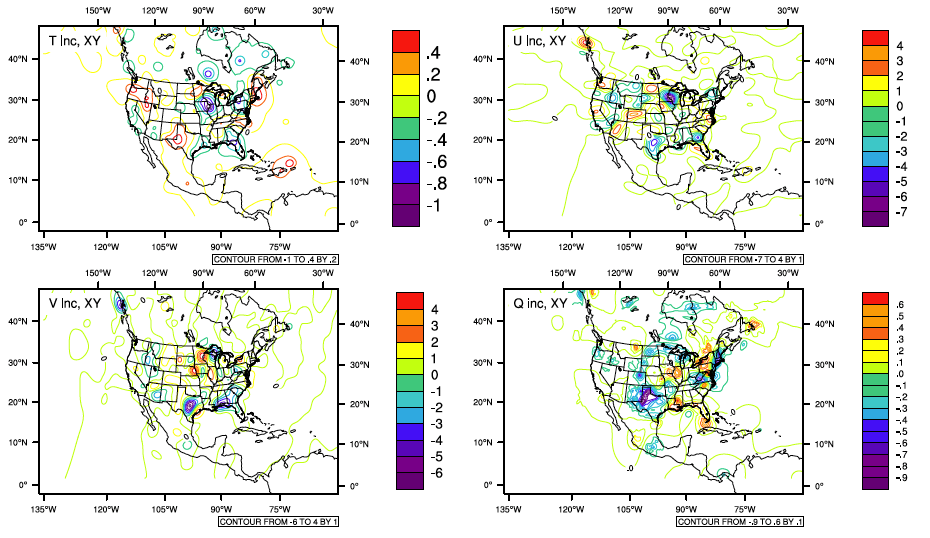
\includegraphics[width=0.9\textwidth]{images/increments}
  \caption{Analysis increment at the 15th level}
  \label{fig:increments}
\end{figure}

The analysis increment indicates that conventional observations are mostly located within the continental United States and that data availability over the ocean is very sparse. 

%-------------------------------------------------------------------------------
\section{Assimilating Radiance Data with Regional GSI}
%-------------------------------------------------------------------------------

%-------------------------------------------------------------------------------
\subsection{Run Script}
\label{sec5.2.1}
%-------------------------------------------------------------------------------

Adding radiance data into the GSI analysis is straightforward after having already run GSI with conventional data.  The same run script from the above section can be used to run GSI with radiance data (with or without PrepBUFR data).  The key step to adding the radiance data is linking the radiance BUFR files to the GSI run directory with the names listed in the \verb|&OBS_INPUT| section of the GSI namelist. The following example adds the two radiance BUFR files:

AMSU-A:   \textit{gdas1.t00z.1bamua.tm00.bufr\_d}\newline
HIRS4:    \textit{gdas1.t00z.1bhrs4.tm00.bufr\_d}

The location of these radiance BUFR files is already included in the scripts variable \verb|OBS_ROOT|, therefore the following two lines can be inserted below the link to the prepBUFR data in the script \textit{run\_gsi\_regional.ksh}:

\begin{scriptsize}
\begin{verbatim}
 ln -s ${OBS_ROOT}/gdas1.t${HH}z.1bamua.tm00.bufr_d amsuabufr
 ln -s ${OBS_ROOT}/gdas1.t${HH}z.1bhrs4.tm00.bufr_d hirs4bufr
\end{verbatim}
\end{scriptsize}

If radiance data is desired in addition to conventional prepBUFR data, the following link to the prepBUFR data should be kept as is:

\begin{scriptsize}
\begin{verbatim}
ln -s ${PREPBUFR} ./prepbufr
\end{verbatim}
\end{scriptsize}

Alternatively, to analyze radiance data without conventional prepBUFR data, this line can be commented out in the script \textit{run\_gsi\_regional.ksh}:

\begin{scriptsize}
\begin{verbatim}
# ln -s ${PREPBUFR} ./prepbufr
\end{verbatim}
\end{scriptsize}

In the following example, both radiance and conventional observations will be assimilated.  

In order to link the correct name for the radiance BUFR file, the namelist section \verb|&OBS_INPUT| should be referenced.  This section has a list of data types and BUFR file names that can be used in GSI.  The 1\textsuperscript{st} column \verb|"dfile"| is the file name recognized by GSI.  The 2\textsuperscript{nd} column \verb|"dtype"| and 3\textsuperscript{rd} column \verb|"dplat"| are the data type and data platform that are included in the file listed in "dfile," respectively. For example, the following line tells us the AMSU-A observation from NOAA-15 should be read from a BUFR file named \textit{"amsuabufr"}:

\begin{scriptsize}
\begin{verbatim}
!  dfile          dtype       dplat     dsis                 dval    dthin dsfcalc
   amsuabufr      amsua       n15       amsua_n15           10.0     2     0
\end{verbatim}
\end{scriptsize}

With radiance data assimilation, data thinning and bias correction need to be checked carefully. The following is a brief description of these two:

\begin{itemize}
\item Radiance data thinning

Radiance data thinning is found in the namelist section \verb|&OBS_INPUT|. The following is a part of namelist in that section:

\begin{scriptsize}
\begin{verbatim}
dmesh(1)=120.0,dmesh(2)=60.0,dmesh(3)=30,time_window_max=1.5,ext_sonde=.true.
!  dfile          dtype       dplat     dsis                 dval    dthin dsfcalc
   amsuabufr      amsua       n15       amsua_n15            10.0     2     0
\end{verbatim}
\end{scriptsize}

The first line of \verb|&OBS_INPUT| lists multiple mesh grids as elements of the array \verb|dmesh| (three mesh grids in the above example). For the line specifying data type, the 2\textsuperscript{nd} to last element of that line is used to specify the choice of \verb|dthin|. This selects the mesh grid to be used for thinning. The data thinning option for NOAA-15 AMSU-A observations is set to 60 km because the value of \verb|dthin| is two, corresponding to \verb|dmesh(2)|=60 km.  For more information about radiance data thinning, please refer to the Advanced GSI User\textquotesingle s Guide.\\

\item Radiance data bias correction

Radiance data bias correction is very important for successful radiance data assimilation.  In the sample run scripts, there are two files related to bias correction:

\begin{scriptsize}
\begin{verbatim}
# for satellite bias correction
cp ${FIX_ROOT}/gdas1.t00z.abias.20150617 ./satbias_in
cp ${FIX_ROOT}/gdas1.t00z.abias_pc.20150617  ./satbias_pc
\end{verbatim}
\end{scriptsize}

For this case, the GDAS bias correction files were downloaded and saved in the fix directory as examples. For other cases, the run script should link to corresponding bias correction coefficient files. The first line sets the path to the bias coefficient file, and the second copies the bias correction coefficients for passive (monitored) channels into the working directory. These two coefficient files are usually calculated from within GSI in the previous cycle. Two files are provided in ./fix as examples of the bias correction coefficients. For the best results, it is necessary for the user to generate his or her own bias files. The details of radiance data bias correction are discussed in the Advanced GSI User\textquotesingle s Guide. Please note that GSI releases prior to v3.5 have coefficients for mass bias correction and angle bias correction calculated separately. \\

Once these links are set, we are ready to run GSI. 


\end{itemize}

%-------------------------------------------------------------------------------
\subsection{Run GSI and Check Run Status}
\label{sec5.2.2}
%-------------------------------------------------------------------------------

The process for running GSI is the same as described in section \ref{sec5.1.2}.  Once \textit{run\_gsi\_regional.ksh} has been submitted, move into the run directory to check the GSI analysis results. For the current case, the run directory will look almost as it did for the conventional data case, the exception being the two links to the radiance BUFR files and new diag files for the radiance data types used. Following the same steps as in section \ref{sec5.1.2}, check the \textit{stdout} file to see if GSI has run through each part of the analysis process successfully.  In addition to the information outlined for the conventional run, the radiance BUFR files should have been read in and distributed to each sub domain: 

\begin{scriptsize}
\begin{verbatim}
OBS_PARA: ps                        1429      3190      4655      6774
OBS_PARA: t                         2564      5200      7057     11128
OBS_PARA: q                         2346      4626      6148      8128
OBS_PARA: pw                          65        80        63        49
OBS_PARA: uv                        3358      6453      8091     11998
OBS_PARA: hirs4     metop-a            0         0      1146      1661
OBS_PARA: hirs4     n19              213      1020         0         0
OBS_PARA: hirs4     metop-b            0         0        85       555
OBS_PARA: amsua     n15             1458      2026       830       234
OBS_PARA: amsua     n18             2223      2318       108         0
OBS_PARA: amsua     n19              176       960         0         0
OBS_PARA: amsua     metop-a            0         0      1077      1559
OBS_PARA: amsua     metop-b            0         0       265      1829
\end{verbatim}
\end{scriptsize}


When comparing this output to the content in step three of section \ref{sec5.1.3}, it can be seen that there are eight new radiance data types that have been read in: HIRS4 from METOP-A, METOP-B and NOAA-19, AMSU-A from NOAA-15, NOAA-18, NOAA-19, METOP-A, and METOP-B.  The table above shows that most of the radiance data read in for this case are AMSU-A from NOAA satellite information.

%-------------------------------------------------------------------------------
\subsection{Diagnose GSI Analysis Results}
%-------------------------------------------------------------------------------

%-------------------------------------------------------------------------------
\subsubsection{Check File fort.207}
%-------------------------------------------------------------------------------

The file \textit{fort.207} contains the statistics for the radiance data, similar to file \textit{fort.203} for temperature.  This file contains important details about the radiance data analysis.  Section \ref{sec4.5.2} explains this file in detail.  Below are some values from the file \textit{fort.207} to provide a quick look at the radiance assimilation for this example. 

The \textit{fort.207} file contains the following lines:

\hspace{4ex} For O-B, before the first outer loop:

\begin{scriptsize}
\begin{verbatim}
    it      satellite instrument     # read     # keep    # assim  penalty      qcpnlty       cpen      qccpen
o-g 01 rad  n15       amsua           83190      58236      25226    10356.       10356.    0.41053    0.41053
o-g 01 rad  n18       amsua           83595      69147      27677    11067.       11067.    0.39988    0.39988
\end{verbatim}
\end{scriptsize}

\hspace{4ex} For O-A, after the second outer loop:

\begin{scriptsize}
\begin{verbatim}
o-g 03 rad  n15       amsua           83190      58236      30136    4672.4       4672.4    0.15504    0.15504
o-g 03 rad  n18       amsua           83595      69147      32253    8546.8       8546.8    0.26499    0.26499
\end{verbatim}
\end{scriptsize}

From the above information, it can be seen that AMSU-A data from NOAA-15 provides 83190 observations within the analysis time window and domain.  After thinning, 58236 observations remained, and only 25226 passed the quality check and were used in the analysis.  The penalty for this data decreased from 10356 to 4672.4 after two outer loops. It is important to note that the number of AMSU-A observations assimilated in the O-A calculation increased to 30136 from 25226 as more data passed the quality check in the 2\textsuperscript{nd} outer loop.
 
The statistics for each channel can be viewed in the \textit{fort.207} file as well.  Here, channels from AMSU-A NOAA-15 are listed as an example:

\hspace{4ex} For O-B, before the first outer loop:

\begin{scriptsize}
\begin{verbatim}
    1    1 amsua_n15          1903     24      3.000   1.6543287  -0.3164878   0.1411234   1.7151923   1.6857402
    2    2 amsua_n15          1927      0      2.200   1.0105548  -0.2430249   0.0385590   1.0284683   0.9993427
    3    3 amsua_n15          1927      0      2.000   1.7941589  -0.1480894   0.0575956   0.7909800   0.7769935
    4    4 amsua_n15          1927      0      0.600  -0.1848763  -0.0460476   0.0856369   0.2497797   0.2454985
    5    5 amsua_n15          1927      4      0.300   0.0314288  -0.0292998   0.3025052   0.2008865   0.1987383
    6    6 amsua_n15          4126     10     -0.230  -1.8448526  -0.0778284   0.8969513   0.2463875   0.2337725
    7    7 amsua_n15          4468     13      0.250  -0.1497841  -0.0810899   0.5245399   0.2042760   0.1874916
    8    8 amsua_n15          4468     13      0.275  -0.0251081  -0.0869918   0.6195120   0.2420568   0.2258847
    9    9 amsua_n15          4463     18      0.340   0.1824903   0.2108491   0.6987405   0.3453174   0.2734717
   10   10 amsua_n15           294   4187      0.400   0.7946961   0.7908103   2.5281681   0.7982470   0.1087077
   15   15 amsua_n15          1922      5      3.500   1.6785936  -0.1471413   0.0940713   1.6461928   1.6396037
\end{verbatim}
\end{scriptsize}

\hspace{4ex} For O-A, after the second outer loop:
 
\begin{scriptsize}
\begin{verbatim}
    1    1 amsua_n15          2050     10      3.000   2.0842622   0.1363398   0.0414276   1.0332965   1.0242622
    2    2 amsua_n15          2060      0      2.200   1.0926873  -0.0731534   0.0177924   0.8048238   0.8014923
    3    3 amsua_n15          2060      0      2.000   1.8733559  -0.0257656   0.0406385   0.6841159   0.6836305
    4    4 amsua_n15          2060      0      0.600  -0.1278763   0.0136412   0.0547146   0.2103718   0.2099291
    5    5 amsua_n15          2060      4      0.300   0.0730860   0.0118626   0.1759475   0.1624923   0.1620587
    6    6 amsua_n15          4234      0     -0.230  -1.7911421  -0.0262042   0.5247873   0.1975867   0.1958414
    7    7 amsua_n15          4470     11      0.250  -0.0766482  -0.0094307   0.1918646   0.1288789   0.1285334
    8    8 amsua_n15          4475      6      0.275   0.0675371  -0.0047226   0.1715888   0.1341703   0.1340871
    9    9 amsua_n15          4481      0      0.340  -0.0508290  -0.0396425   0.1722334   0.1711928   0.1665396
   10   10 amsua_n15          4362    119      0.400   0.2373520   0.1943598   0.3425567   0.3140220   0.2466457
   15   15 amsua_n15          2058      2      3.500   1.8261335   0.0617429   0.0487809   1.2317674   1.2302190
\end{verbatim}
\end{scriptsize}

The second column is the channel number for AMSU-A and the last column is the standard deviation for each channel.  It can be seen that most of the channels fit better to the observations after the second outer loop. 

%-------------------------------------------------------------------------------
\subsubsection{Check the Analysis Increment}
%-------------------------------------------------------------------------------

The same methods for checking the optimal minimization as demonstrated in section \ref{sec5.1.4.2} can be used for radiance assimilation.  Similar features to the conventional assimilation should be seen with the minimization. The figures below show detailed information on how the radiance data impact the analysis results on top of the conventional data.  Using the same NCL script as in section \ref{sec5.1.4.3}, analysis increment fields are plotted comparing the analysis results with radiance and conventional data to the analysis results with conventional data assimilation only.  Figure \ref{fig:increments_rad2} is for vertical level 49 and Figure \ref{fig:increments_rad} is for vertical level six, representing the maximum temperature increment level (49) and maximum moisture increment level (6), respectively.  

\begin{figure}[h!]
  \centering
  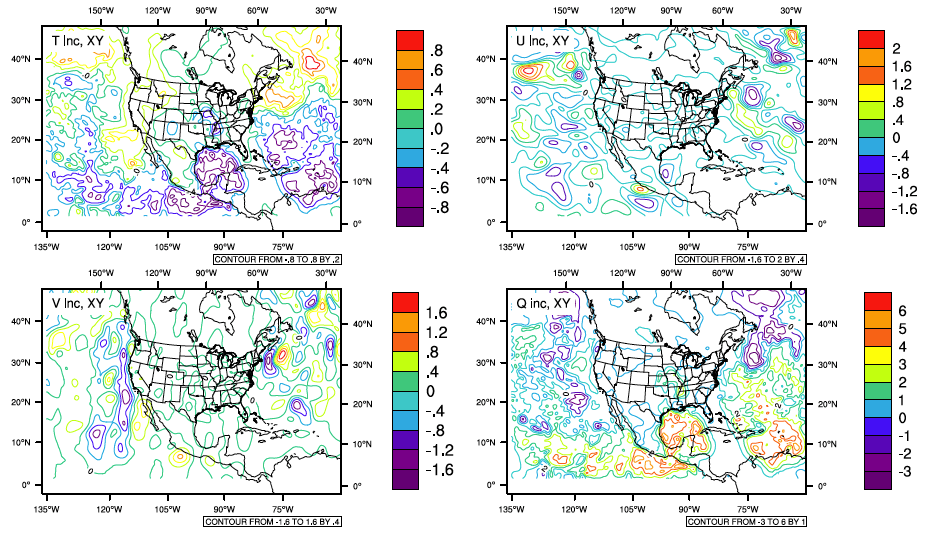
\includegraphics[width=0.9\textwidth]{images/increments_rad}
  \caption{Analysis increment fields of the prepBUFR and radiance data analysis compared to the analysis with prepBUFR only at vertical level six}
  \label{fig:increments_rad}
\end{figure}

\begin{figure}[h!]
  \centering
  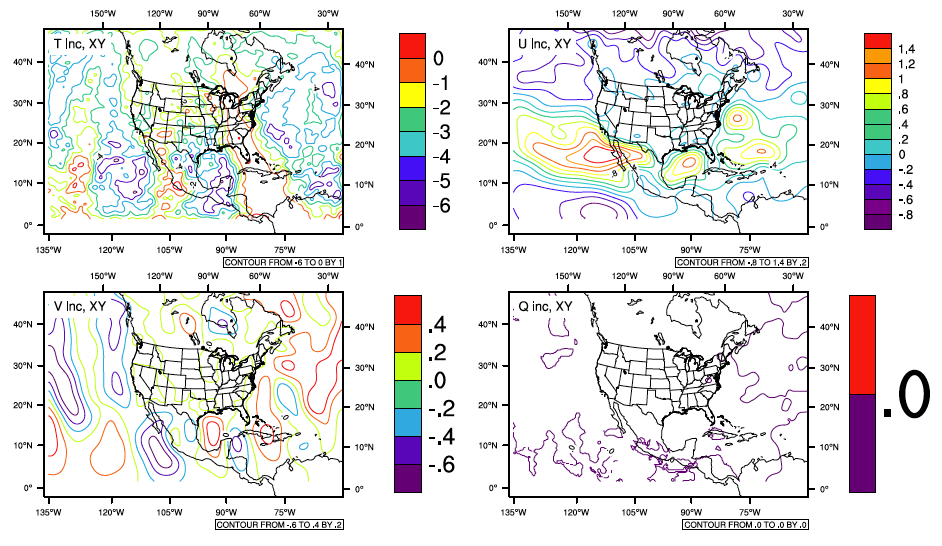
\includegraphics[width=0.9\textwidth]{images/increments_rad2}
  \caption{Analysis increment fields of the prepBUFR and radiance data analysis compared to the analysis with prepBUFR only at vertical level 49}
  \label{fig:increments_rad2}
\end{figure}

In order to fully understand the analysis results, the following topics should be reviewed:

\begin{enumerate}
\item The weighting functions of each channel and the data coverage at the analysis time.  There are several sources on the internet that show the weighting functions of the AMSU-A channels. Channel one is the moisture channel, while the others are mainly temperature channels (Channels two, there, and 15 also have large moisture signals).  Because a model top of 20 mb was specified for this case study, the actual impact should come from channels with peak weighting below 20 hPa.

\item The usage of each channel is located in the file named \textit{'satinfo'} in the run directory.  The first two columns show the observation type and platform of the channels, and the third column indicates if the channel is used in the analysis.  Because many amsua\_n15 and amsua\_n18 data were used, they should be checked in detail.  In this case, Channels six, 11, and 14 from amsua\_n15 and channels nine and 14 from amsua\_n18 were turned off. 

\item Thinning information, including a quick look at the namelist in the run directory. The file "gsiparm.anl" shows that both amsua\_n15 and amsu\_n18 use thinning grid two, which is 60 km.  In this case, the grid spacing is 30 km, which indicates to use the satellite observations every four grid-spaces, which might be a little dense. 

\item Bias correction: Radiance bias correction was previously discussed. It is very important for a successful radiance data analysis. The run script can only link to the GDAS bias correction coefficients that are provided as an example in \textit{./fix}:

\begin{scriptsize}
\begin{verbatim}
cp ${FIX_ROOT}/gdas1.t00z.abias.20150617 ./satbias_in
cp ${FIX_ROOT}/gdas1.t00z.abias_pc.20150617  ./satbias_pc
\end{verbatim}
\end{scriptsize}

Users can download the operational bias correction coefficients during their experiment period as a starting point to calculate the coefficients suitable for their experiments. \\

Radiance bias correction for regional analyses is a difficult issue because of the limited coverage of radiance data.  This topic is out of the scope of this document, but this issue should be considered and understood when using GSI with radiance applications. 
\end{enumerate}

%-------------------------------------------------------------------------------
\section{Assimilating GPS Radio Occultation Data with Regional GSI}
%-------------------------------------------------------------------------------

%-------------------------------------------------------------------------------
\subsection{Run Script}
%-------------------------------------------------------------------------------

The addition of GPS Radio Occultation (RO) data into the GSI analysis is similar to that of adding radiance data. In the example below, the RO data is used as refractivity.  There is also an option to use the data as bending angles. The same run scripts in sections \ref{sec5.1.1} and \ref{sec5.2.1} can be used with the addition of the following link to RO observations:

\begin{scriptsize}
\begin{verbatim}
 ln -s ${OBS_ROOT}/gdas1.t${HH}z.gpsro.tm00.bufr_d gpsrobufr
\end{verbatim}
\end{scriptsize}

For this case study, the GPS RO BUFR file was downloaded and saved in the \verb|OBS_ROOT| directory.  The file is linked to the name \textit{gpsrobufr}, following the namelist section \verb|&OBS_INPUT|:

\begin{scriptsize}
\begin{verbatim}
!  dfile          dtype       dplat     dsis                 dval    dthin dsfcalc

   gpsrobufr      gps_ref     null      gps                  1.0     0     0
\end{verbatim}
\end{scriptsize}
This indicates that GSI is expecting a GPS refractivity BUFR file named \textit{gpsrobufr}.  In the following example, GPS RO and conventional observations are both assimilated.  Change the run directory name in the run scripts to reflect this test:

\begin{scriptsize}
\begin{verbatim}
WORK_ROOT=/scratch1/gsiprd_${ANAL_TIME}_gps_prepbufr
\end{verbatim}
\end{scriptsize}

%-------------------------------------------------------------------------------
\subsection{Run GSI and Check the Run Status}
%-------------------------------------------------------------------------------

The process of running GSI is the same as described in section \ref{sec5.1.2}.  Once \textit{run\_gsi\_regional.ksh} has been submitted, move into the working directory, \textit{gsiprd\_2014061700\_gps\_prepbufr}, to check the GSI analysis results.  The run directory will look exactly the same as with the conventional data, with the exception of the link to the GPS RO BUFR files used in this case. Following the same steps as in section \ref{sec5.1.3}, check the standard output file to see if GSI has run through each part of the analysis process successfully.  In addition to the information outlined for the conventional run, the GPS RO BUFR files should have been read in and distributed to each sub domain:

\begin{scriptsize}
\begin{verbatim}
OBS_PARA: ps                        1429      3190      4655      6774
OBS_PARA: t                         2564      5200      7057     11128
OBS_PARA: q                         2346      4626      6148      8128
OBS_PARA: pw                          65        80        63        49
OBS_PARA: uv                        3358      6453      8091     11998
OBS_PARA: gps_ref                   1799      1368      2664      3520
\end{verbatim}
\end{scriptsize}

Comparing the output to the content in section \ref{sec5.1.3}, it can be seen that the GPS RO refractivity data have been read in and distributed to four sub-domains successfully.

%-------------------------------------------------------------------------------
\subsection{Diagnose GSI Analysis Results}
%-------------------------------------------------------------------------------

%-------------------------------------------------------------------------------
\subsubsection{Check File \textit{fort.212}}
%-------------------------------------------------------------------------------

The file \textit{fort.212} shows the fit of the analysis/background to the GPS/RO data as fractional differences.  It has the same structure as the fit files for conventional data.  Below is a quick look to be sure the GPS RO data were used:

\begin{tiny}
\begin{verbatim}
  Observation - Background (O-B)

                              ptop   1000.0    900.0    800.0    600.0    400.0    300.0    250.0    200.0    150.0    100.0     50.0      0.0
     it     obs    type styp  pbot   1200.0   1000.0    900.0    800.0    600.0    400.0    300.0    250.0    200.0    150.0    100.0   2000.0
----------------------------------------------------------------------------------------------------------------------------------------------
 o-g 01             all      count        0       13       58      223      355      342      232      261      326      440      729     3740
 o-g 01             all       bias     0.00    -0.76    -0.03    -0.06    -0.04     0.01    -0.03     0.04    -0.04    -0.16    -0.18    -0.14
 o-g 01             all        RMS error     0.00     1.41     0.75     0.96     0.79     0.35     0.32     0.42     0.54     0.57     0.55     0.59

  Observation - Analysis (O-A)

                              ptop   1000.0    900.0    800.0    600.0    400.0    300.0    250.0    200.0    150.0    100.0     50.0      0.0
     it     obs    type styp  pbot   1200.0   1000.0    900.0    800.0    600.0    400.0    300.0    250.0    200.0    150.0    100.0   2000.0
----------------------------------------------------------------------------------------------------------------------------------------------
 o-g 03             all      count        1       18       65      229      355      342      231      266      330      440      731     3776
 o-g 03             all       bias    -0.40    -0.43     0.03     0.02    -0.02    -0.01    -0.02     0.00     0.01    -0.01    -0.02     0.00
 o-g 03             all        RMS error     0.40     1.03     0.54     0.59     0.70     0.26     0.14     0.20     0.24     0.28     0.39     0.41
\end{verbatim}
\end{tiny}

It can be seen that most of the GPS RO data are located in the upper levels, with a total of 3740 observations used in the analysis during the 1\textsuperscript{st} outer loop, and 3776 used to calculate O-A. After the analysis, the data bias reduced from -0.14 to 0.00, and the RMS error was reduced from 0.59 to 0.41. It can be concluded that the analysis with GPS RO data looks reasonable from these statistics.  

%-------------------------------------------------------------------------------
\subsubsection{Check the Analysis Increment}
%-------------------------------------------------------------------------------

The same methods for checking the minimization in section \ref{sec5.1.4.2} can be used for the GPS RO assimilation. 

The following figures provide detailed information about how the new data impacts the analysis.  Using the NCL script from section \ref{sec5.1.4}, analysis increment fields are plotted comparing the analysis results with GPS RO and conventional data to the analysis results with conventional data assimilation only for vertical level 48, which represents the maximum temperature increment.  

\begin{figure}[h!]
  \centering
  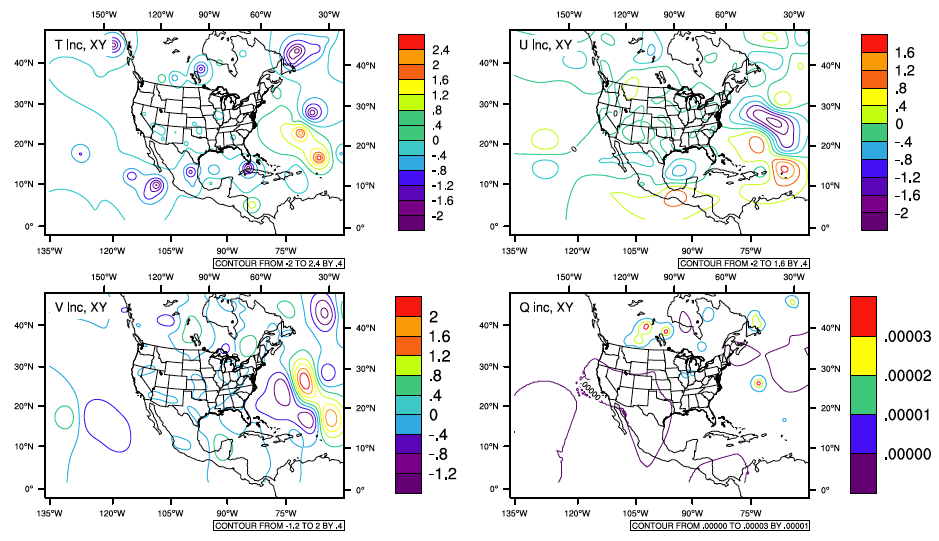
\includegraphics[width=0.9\textwidth]{images/increments_bufr}
  \caption{Analysis increment fields comparing the use of GPS RO and conventional observations to only prepBUFR at vertical level 48.}
  \label{fig:increments_bufr}
\end{figure}

%-------------------------------------------------------------------------------
\section{Introduction to GSI Hybrid 3DEnVar Analysis}
%-------------------------------------------------------------------------------

The three-dimensional hybrid ensemble-variational (hybrid 3DEnVar) analysis is an important option in the GSI system that has been used operationally. It provides the ability to bring the flow dependent background error covariance into the analysis based on ensemble forecasts. If ensemble forecasts have been generated, setting up GSI to do a hybrid analysis is straightforward and only requires two changes in the run script in addition to the current 3DVAR run script:

\begin{itemize}[leftmargin=*]
\item \textit{Change 1: Link the ensemble members to the GSI run directory}\\

This change is required to link the ensemble members to the GSI run directory and assign each ensemble member a name that GSI recognizes. GSI can accept four kinds of ensemble forecasts, controlled by the namelist variable \textit{regional\_ensemble\_option}. Table \ref{tab51} provides a list of options for \textit{regional\_ensemble\_option} and the naming convention for linking the ensemble files to GSI recognized names. \\


\begin{table}[htbp]
\centering
\begin{small}
\caption{List of ensemble forecasts that can be read by GSI}
\begin{tabular}{|p{1.7cm}|p{4cm}|p{4.6cm}|p{4cm}|}
\hline
\hline
regional\_ ensemble\_ option & explanation & Function called & GSI recognized  ensemble file names \\
\hline
1 & GFS ensemble internally interpolated to hybrid grid & get\_gefs\_for\_regional & \textit{filelist : a text file including the path and name of ensemble files} \\
\hline
2 & Ensemble is in WRF-NMM (HWRF) format & get\_wrf\_nmm\_ensperts & 
\textit{d01\_en001},\newline \textit{d01\_en002},\newline ... \\
\hline
3 & Ensemble is in ARW netcdf format & get\_wrf\_mass\_ensperts\_netcdf & 
\textit{wrf\_en001}, \newline 
\textit{wrf\_en002}, \newline ... \\
\hline
4 & Ensemble is in NMMB format & get\_nmmb\_ensperts &
 \textit{nmmb\_ens\_mem001},\newline
  \textit{nmmb\_ens\_mem002},\newline ...\\
\hline
\end{tabular}
\label{tab51}
\end{small}
\end{table} 


Users have to change the GSI run script to add the links to the ensemble forecasts if they want to use the GSI hybrid function. Below is an example of using an ensemble in ARW netcdf format, assuming that all the ensemble members are located in a directory defined by the parameter \textit{\${mempath}} and the ensemble members have a name such as: \textit{wrfout\_d01\_\${iiimem}}, where \textit{\${iiimem}} is an integer indicating the ensemble member ID. The following lines should be added to the run script with loop \textit{iiimem} from one to the total number of ensemble members:

\begin{scriptsize}
\begin{verbatim}
	if [ -r  ${mempath}/wrfout_d01_${iiimem} ]; then
   ln -sf ${mempath}/wrfout_d01_${iiimem} ./wrf_en${iiimem}
	else
   echo "member ${mempath}/wrfout_d01_${iiimem} does not exit"
	fi
\end{verbatim}
\end{scriptsize}

\item \textit{Change 2: Set up the namelist options in section HYBRID\_ENSEMBLE}\\

Users need to set \verb|l_hyb_ens=.true.| to turn on the hybrid ensemble analysis. Commonly used namelist options for the hybrid analysis are listed in table \ref{tab52}:

\begin{table}[htbp]
\centering
\caption{The list of namelist options for GSI hybrid}
\begin{tabular}{|p{3cm}|p{11cm}|}
\hline
Options & explanation \\
\hline
l\_hyb\_ens &  if true, turn on hybrid ensemble option \\
\hline
uv\_hyb\_ens & if true, ensemble perturbation wind variables are u and v; \newline
otherwise, ensemble perturbation wind variables are stream function and velocity potential \\
\hline
generate\_ens &  if true, generate an internal ensemble based on the existing background error; recommended = false \\
\hline
n\_ens &  number of ensemble members \\
\hline
beta1\_inv& (1/beta1), the weight given to the static background error covariance. 0 <= beta1\_inv <= 1, should be tuned for optimal performance; beta2\_inv = 1 - beta1\_inv is the weight given to the ensemble derived covariance \newline
=1, ensemble information turned off \newline
=0, static background errors turned off \\
\hline
s\_ens\_h & homogeneous isotropic horizontal ensemble localization scale (km) \\
\hline
s\_ens\_v &  vertical localization scale \newline
If positive, in grid units; \newline
if negative, in lnp unit \\
\hline
regional\_ensemble\newline
\_option & integer, used to select the type of ensemble to read in for regional applications. Currently takes values from one to four: \newline
	=1: use GEFS internally interpolated to ensemble grid; \newline
	=2: ensembles are in WRF-NMM format; \newline
	=3: ensembles are in ARW netcdf format; \newline
	=4: ensembles are in NMMB format. \\
\hline
grid\_ratio\_ens & for regional runs, the ratio of ensemble to analysis grid resolution. If turned on and specified with an appropriate value, this could increase the computational efficiency. \\
\hline
\end{tabular}
\label{tab52}
\end{table} 

Please note: the parameters \verb|s_ens_h|, \verb|s_ens_v|, and \verb|beta1_inv| are tunable parameters. They should be tuned for best performance.\\

After setting up the namelist parameters and the path/name of the ensemble members, GSI can be run in the same manner as the other 3DVAR cases introduced in this chapter.  The same procedures could be followed as in the previous sections to check the run status and diagnose the GSI analysis.

\end{itemize}

\newpage
%-------------------------------------------------------------------------------
\section{Introduction to GSI Hybrid 4DEnVar Analysis}
%-------------------------------------------------------------------------------

The GSI hybrid 4DEnVAR analysis is similar to the hybrid 3DEnVar except that the hybrid 4DEnVar will use multiple background files and GFS ensemble forecasts. As an example, the following shows how to conduct a hybrid 4DEnVar analysis using three time levels of background files and ensembles.

Before creating a hybrid 4DEnVar analysis, be sure to read the previous section about how to run hybrid 3DEnVar first. The following steps are additional procudures beyond hybrid 3DEnVar and assume that all hybrid 3DEnVar settings have already been set. 

(1). Set \textit{if\_4DEnVar=Yes} in \textit{run\_gsi\_regional.ksh}. 

(2). Set the correct background files and ensemble files at different time levels in \textit{run\_gsi\_regional.ksh}. See the following example:
\begin{scriptsize}
\begin{verbatim}
      if [ ${if_4DEnVar} = Yes ] ; then
        BK_FILE_P1=${BK_ROOT}/wrfout_d01_2017-05-13_19:00:00
        BK_FILE_M1=${BK_ROOT}/wrfout_d01_2017-05-13_17:00:00

        ENSEMBLE_FILE_mem_p1=${ENS_ROOT}/sfg_2017051312_fhr09s
        ENSEMBLE_FILE_mem_m1=${ENS_ROOT}/sfg_2017051312_fhr03s
      fi
\end{verbatim}
\end{scriptsize}

  Note that the background file at the analysis time (201705131800 for the above example) is set by \textit{BK\_FILE} and the ensemble files at the analysis time are set by \textit{ENSEMBLE\_FILE\_mem} as introduced in previous sections. See the following example:

\begin{scriptsize}
\begin{verbatim}
 BK_FILE=${BK_ROOT}/wrfout_d01_2017-05-13_18:00:00
 ...
 if [ ${if_hybrid} = Yes ] ; then
 ...
   ENSEMBLE_FILE_mem=${ENS_ROOT}/sfg_2017051312_fhr06s 
 ...
\end{verbatim}
\end{scriptsize}

Now GSI can be run following the hybrid 3DEnVar case introducted in the prevous section. Similar procedures can be conducted to check the GSI run status and results.

%-------------------------------------------------------------------------------
\section{Summary}
%-------------------------------------------------------------------------------

This chapter applied previous information outlined in the user\textquotesingle s guide to demonstrate how to set up, run, and analyze GSI for various regional applications.  It is important to always check for a successful GSI analysis, as running to completion does not always indicate a successful analysis was generated.  Using the tools and methods described in this chapter, a complete picture of the GSI analysis can be obtained. 

It is important to realize that GSI applications are not limited to regional analyses with WRF. Other GSI applications, including global analyses for GFS, chemical analyses, and others will be introduced in the next chapter.
